\section{Methode}\label{cha:method}

In diesem Kapitel wird der Entwicklungsprozess des auf \textit{CNN}s basierenden Pilzerkennungsalgorithmus behandelt (siehe Kapitel \ref{cha:intr:aim}). Vorerst wird auf den Datenbeschaffungsprozess sowie die Datenvorverarbeitung eingegangen. Die darauf folgenden Abschnitte behandeln den Optimierungsprozess der \textit{Meta-Parameter} (siehe Kapitel \ref{cha:theo:backprop}, \ref{cha:theo:cnn} \& \ref{cha:theo:mod}) und erwähnen kurz diejenigen Massnahmen, welche zu einer signifikanten Verbesserung der Leistung des Erkennungsalgorithmus führten.

In diesem Projekt wird für die Datenaufbereitung der Trainingsdaten wie auch für das Erstellen und Trainieren von \textit{KNN}s die Entwicklungsumgebung MatLab mit der \textit{Deep Learning Toolbox}\cite{matlab} verwendet. Die Entscheidung fiel auf MatLab aufgrund des effizienten und einfach zu modifizierenden Grundgerüstes für \textit{Deep Learning} und \textit{KNN}s. Die Unterstützung von Mehrkernprozessoren sowie die Einbindung von Grafikkarten beschleunigt zudem den Trainingsprozess merklich. Auch sind in MatLab vortrainierte \textit{KNN}s für das \textit{Transfer-Learning} (siehe Kapitel \ref{cha:theo:mod:tl}) einfach zu implementieren und modifizieren.

\subsection{Datenbeschaffung} \label{cha:met:datagathering}
Trainingsdaten bilden die Grundlage jedes auf \textit{Machine Learning} basierenden Algorithmus, weswegen man ein solides Fundament aus vielen Trainingsdaten benötigt (siehe Kapitel \ref{cha:theo:ml:training}). Da die Datenlage für Pilzbilder hingegen eher schlecht ist, ist die Datenbeschaffung ein wichtiger Bestandteil dieser Arbeit. Dabei gilt es, möglichst viele korrekt bestimmte Pilzbilder zu sammeln.

Für das Training sollen von jeder der 20 ausgewählten Pilzarten (siehe Tabelle \ref{table:shrooms}) mindestens 230 verschiedene Bilder beschaffen werden, von den unbekannten 1840 (das Achtfache). Um die Leistung des Algorithmus mittels unabhängigen Daten zu testen (siehe \textit{Validierung} in Kapitel \ref{cha:theo:ml:b-v}), werden zusätzlich 20 Bilder pro bekannte Art resp. 160 für die unbekannte Kategorie gesammelt. Somit mussten 250 Bilder pro ausgewählte Art sowie 2000 Bilder von unbekannten Arten gesammelt werden, insgesamt also etwa 7000 Bilder. Die Anzahl der bekannten Arten begründet sich mit den schwer verfügbaren Bilddaten, die der unbekannten durch eine erfahrungsgestützte Abschätzung, um im Rahmen einer Maturarbeit zu bleiben und trotzdem noch aussagekräftige Ergebnisse erhalten zu können.

Folgende Massnahmen wurden ergriffen, um möglichst viele, reine Trainingsdaten zu beschaffen:

\subsubsection{Datenbank SwissFungi}
Um einen Grunddatensatz zu erhalten, wurde die Fotodatenbank vom offiziellen SwissFungi Pilzatlas der WSL Schweiz verwendet\cite{wsl}. Von den 20 ausgewählten Arten konnten dadurch je einige Dutzend Bilder gesammelt werden; von den unbekannten Arten konnte die geforderte Anzahl von 2000 Exemplaren gedeckt werden. Diese Bilder sind alle professionell bestimmt und bedürfen daher keiner weiteren Kontrolle um die Datenreinheit zu garantieren. 

\subsubsection{Webseite ShroomNET}
Um Pilzsammler und Pilzfotografen aus der Region einfach zu erreichen, wurde die Webseite \textit{www.obermeier.ch} mit einem Hochladeformular für Pilzbilder eingerichtet. Aus einer Liste der ausgewählten Arten lässt sich die Kategorie auswählen, wobei die hochzuladenden Bilder mittels Drag-and-Drop direkt hochgeladen werden. Neben der Hochladefunktion wurde um die Datenreinheit zu gewährleisten zusätzlich ein \textit{Quiz} erstellt, bei dem Besucher die hochgeladenen Pilzbilder klassifizieren können. Mithilfe dieser Webseite lassen sich somit einfach weitere Bilder zusammentragen, welche auch direkt von erfahrenen Sammlern verifiziert werden können (siehe Abbildung \ref{img:webpage}).

Verbreitet wurde die Webseite über Telefonate und Mail-Verkehr mit Pilzkontrolleuren aus der Region Brugg-Aarau sowie in einem Artikel der Schweizerischen Zeitschrift für Pilzkunde SZP\cite{szp}, welche in der ganzen Schweiz versendet wurde. Mittels der Webseite konnten nochmals insgesamt etwa 300 Bilder gesammelt werden.

\subsubsection{Internet Crawler}
Mithilfe eines Python-Skriptes\cite{crawler} konnten automatisiert mit der Google-Suchmaschine nochmals etwa 400 Bilder pro Art gefunden und heruntergeladen werden, gesucht wurde dabei nach dem wissenschaftlichen Namen der Pilze (siehe Tabelle \ref{table:shrooms} im Anhang). Aufgrund vieler Unreinheiten waren pro Kategorie nur etwa 150 weitere Bilder brauchbar. Da die Google-Suche nicht immer korrekte Ergebnisse liefert, wurden diese Bilder auf die Webseite hochgeladen, um sie im \textit{Quiz} nochmals von Pilzsammlern verifizieren zu lassen. 

\subsubsection{Videos}
Eine weitere Möglichkeit, um an viele Bilddaten zu kommen, ist das Extrahieren von Standbildern aus Videos. Bei sich ändernden Kameraperspektive lassen sich mehrere Standbilder von selben Pilz anfertigen, welche nicht identisch sind und sich daher als Trainingsdaten eignen. Dafür wurde das von Michael Bachmeier\cite{bachmeier} zur Verfügung gestellte Videomaterial verwendet. Insgesamt liessen sich durch die Bearbeitung von Videos weitere 1500 Bilder zur Datenbank hinzufügen. Auch diese Daten bedürfen aufgrund der zuverlässigen Quelle keiner weiteren Kontrolle.

\begin{figure}[h]
	\centering
	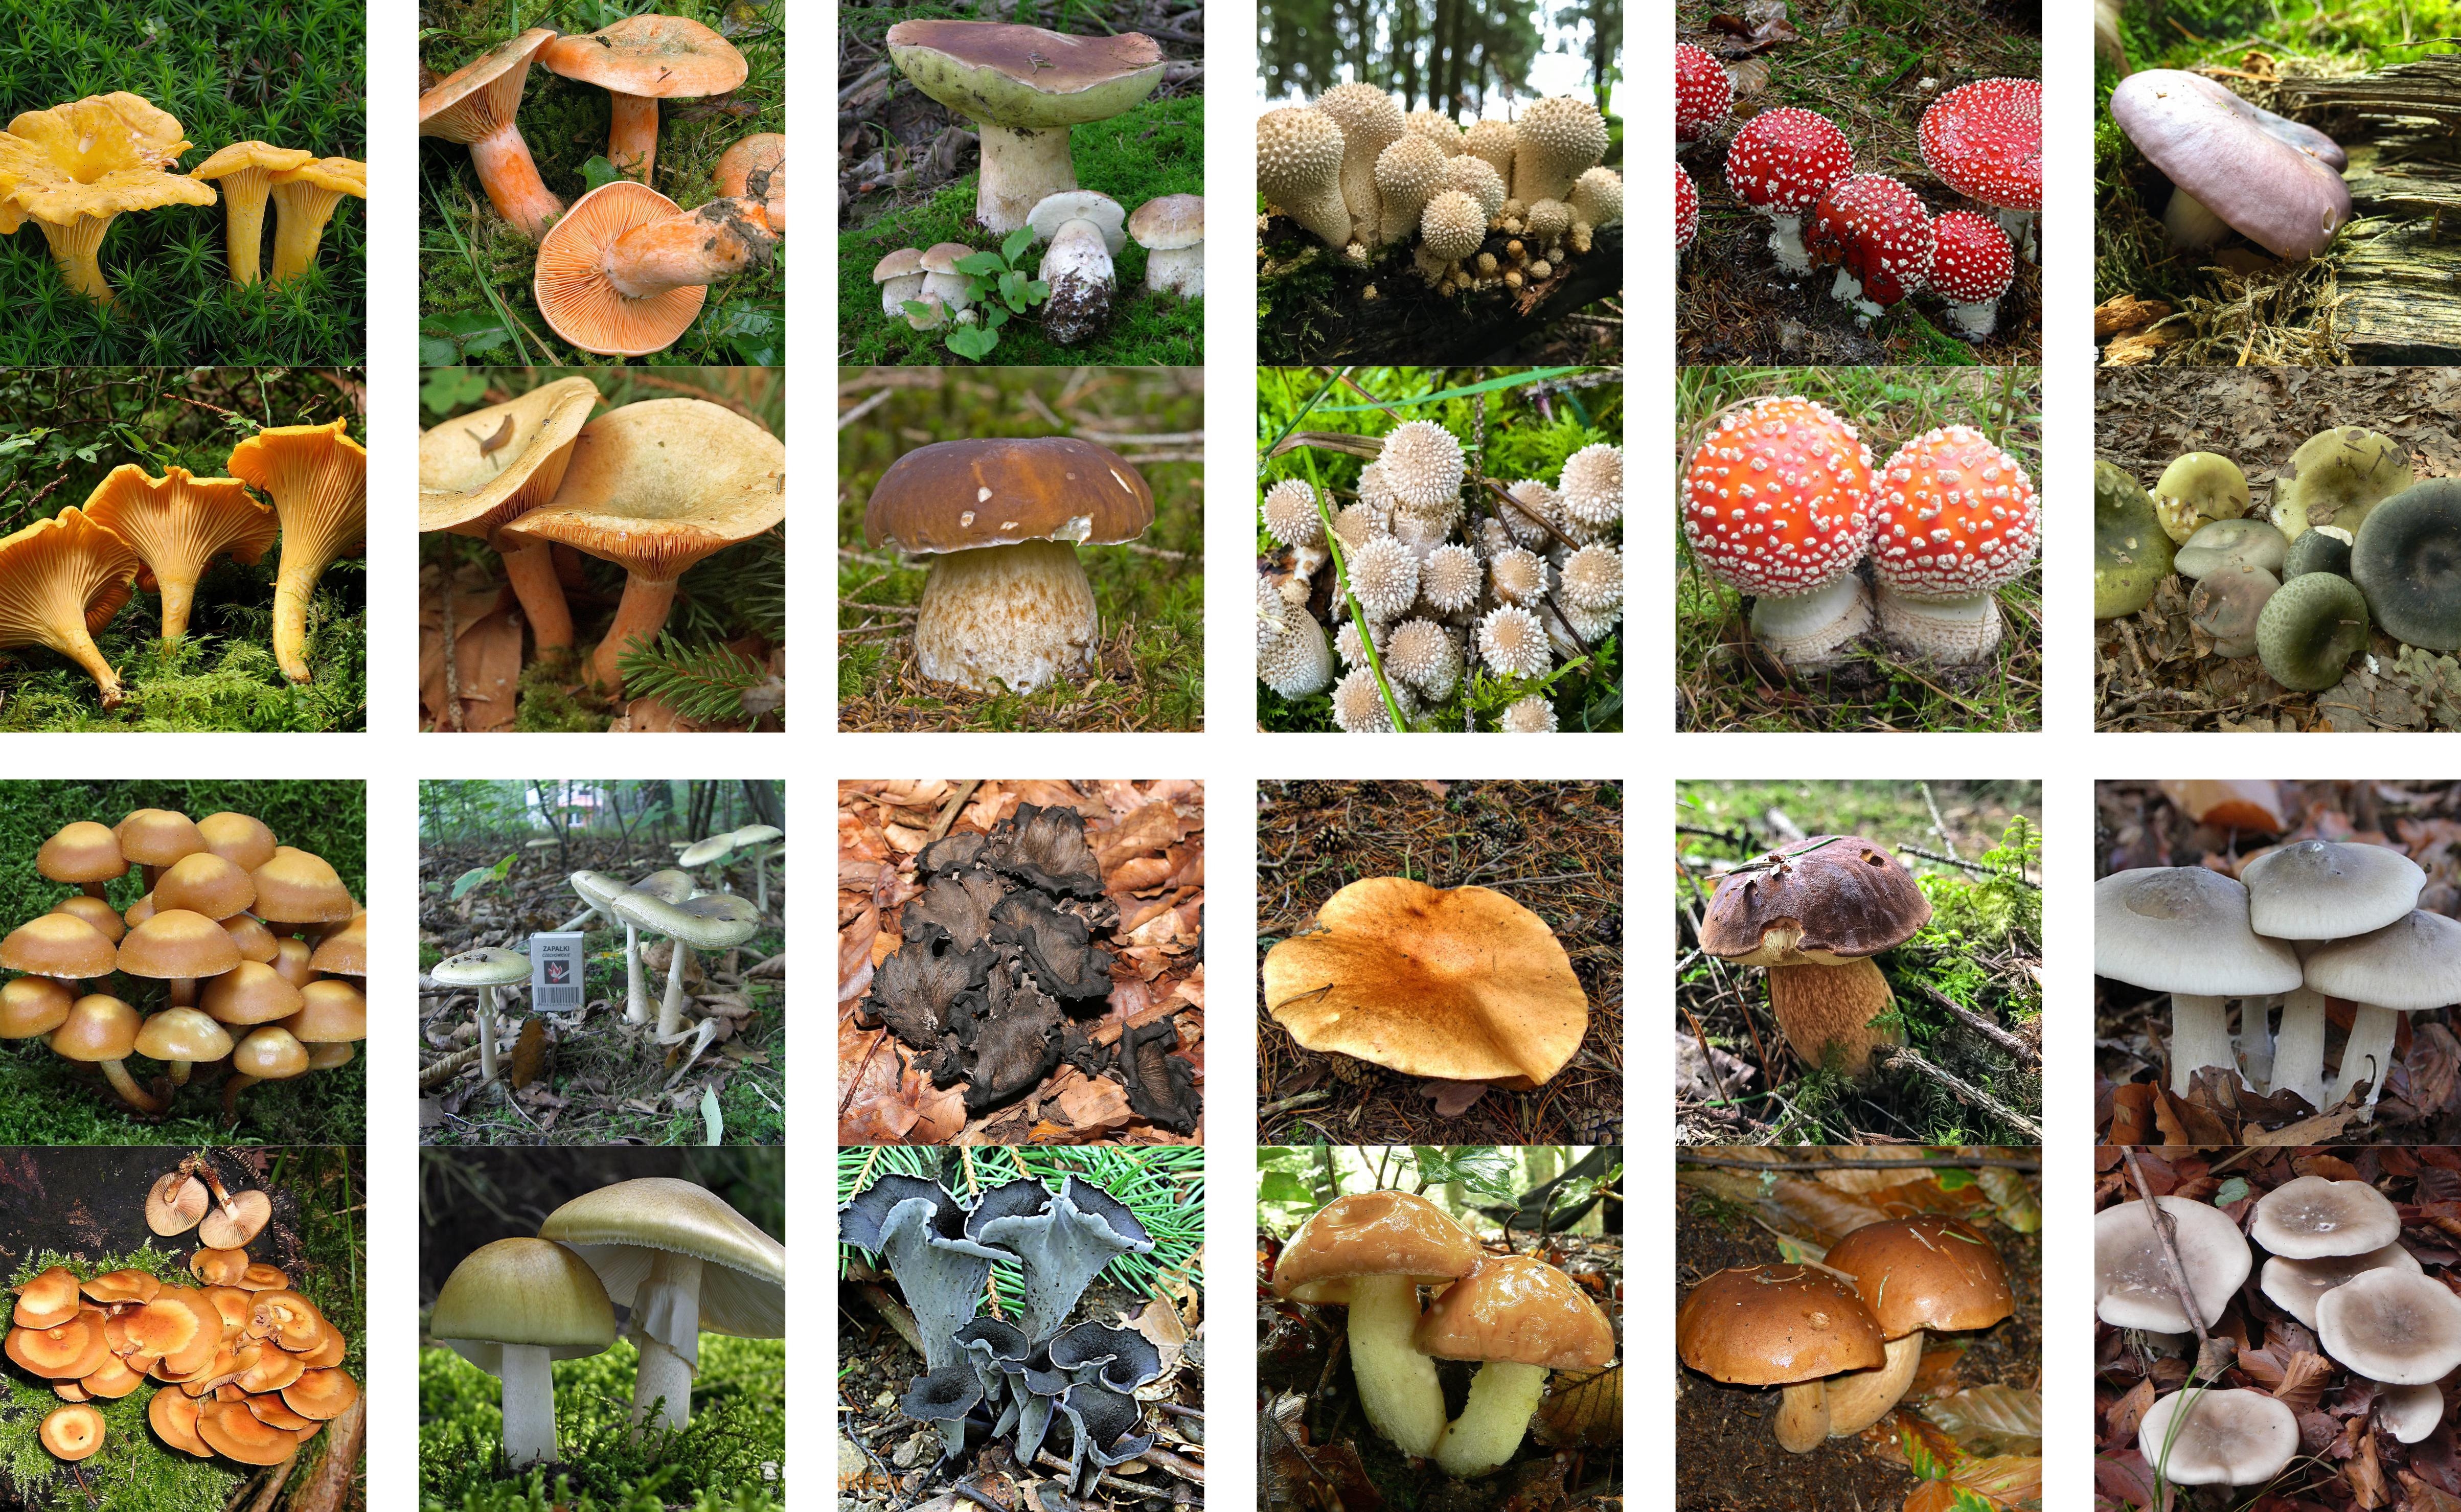
\includegraphics[width=\textwidth]{imgs_raw}
	\caption[Rohdaten]{Beispielbilder von gesammelten Rohdaten der ersten 12 ausgewählten Pilzarten}
	\label{img:raw_imgs}
\end{figure}

\newpage

\subsection{Datenaufbereitung} \label{cha:met:preprocessing}
Nach dem Sammeln der rohen Bilddaten gilt es in der Aufbereitung darum, diese durch einige Vorverarbeitungsmethoden auf das Training anzupassen.

\subsubsection{Bildbearbeitung}
Im ersten Schritt der Datenaufbereitung wurden die Eingangsdaten durch Zentrieren sowie Skalieren auf den Pilz zugeschnitten\footnote{Zwar könnten die Daten auch unbearbeitet in das Training eingespeist werden, jedoch erschwert die zusätzliche Lokalisierung des Pilzes den Lernprozess und führt unweigerlich zu einer Verschlechterung der Erkennungsleistung. Das Problem der Objektfindung in Bildern soll nicht Teil der Problemstellung sein, weswegen dieser Schritt hier manuell verrichtet wird.}. Dafür wurde eine Mindestauflösung von $200 \times 200$px festgelegt, welches eine gute Balance zwischen Details im Bild und Komplexität des Netzes bildet. Ein zu diesem Zwecke mit MatLab programmiertes Hilfsprogramm (siehe Abbildung \ref{img:precrocessing}) beschleunigte den manuellen Bearbeitungsprozess von Bildern wie auch Videos.

\begin{figure}[h]
	\centering
	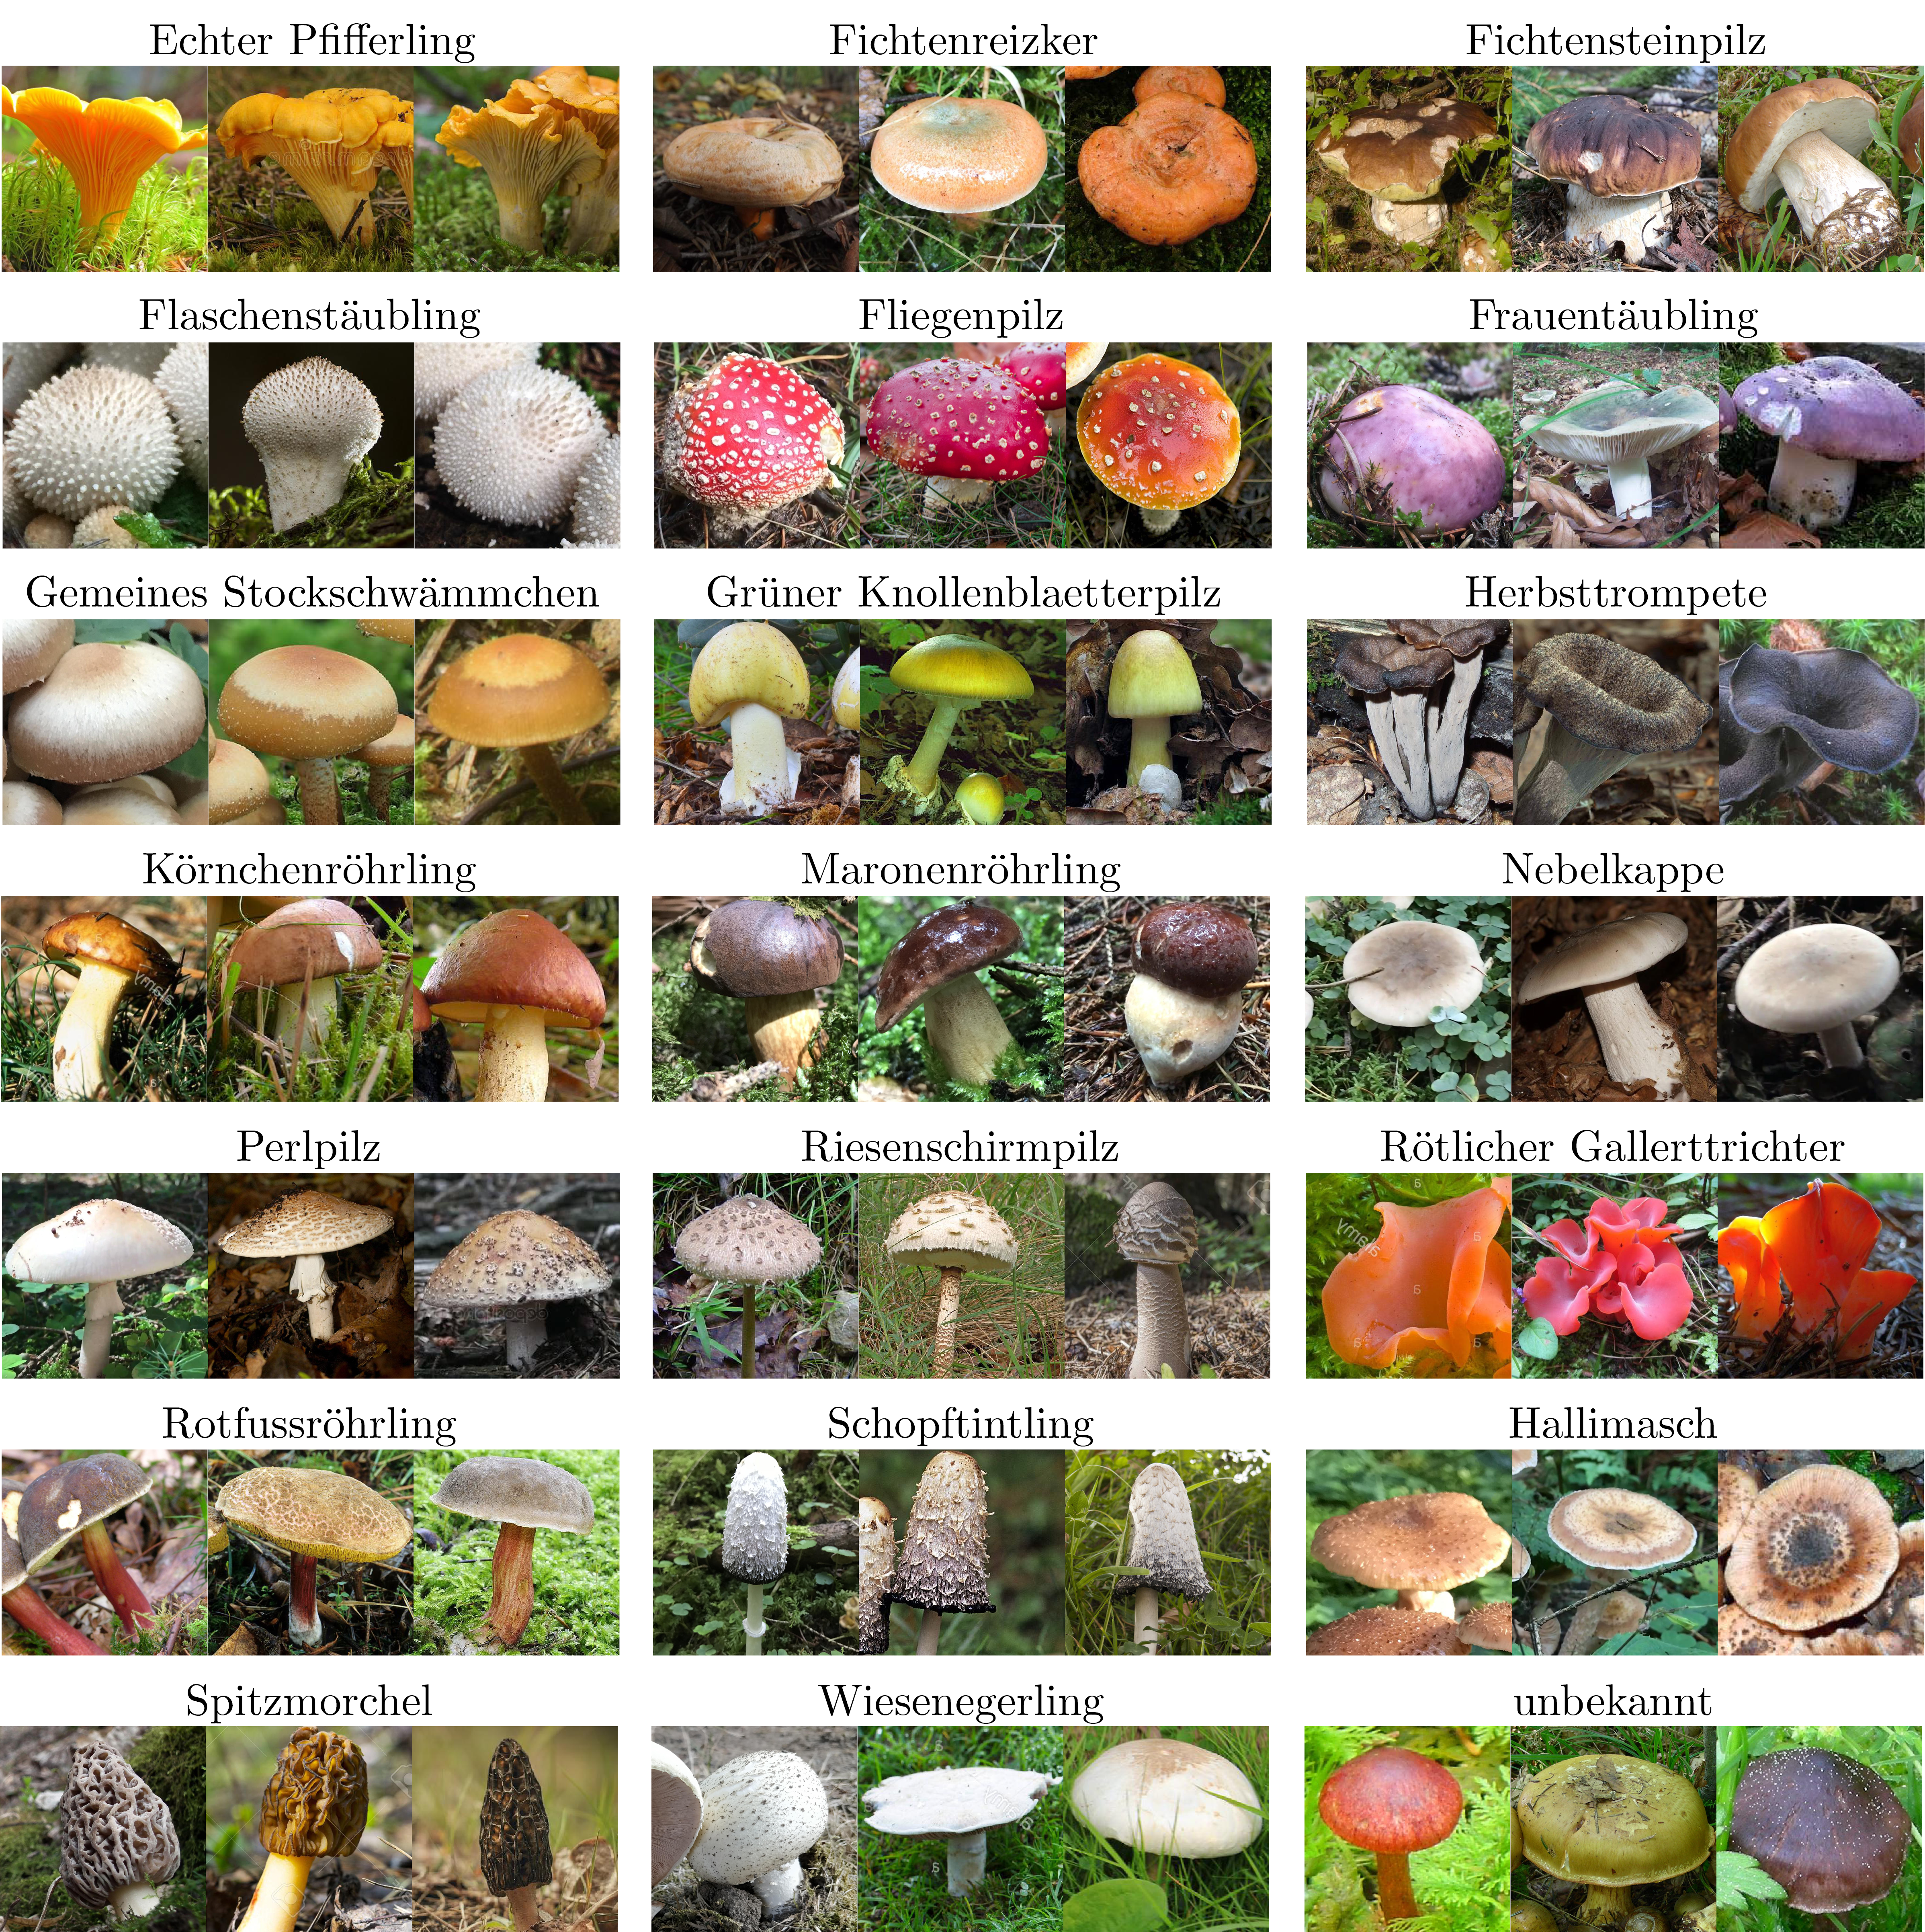
\includegraphics[width=\textwidth]{imgs_cropped_3}
	\caption[\textit{Beispiele Trainingsbilder}]{Je drei bearbeitete Beispielbilder aus den 21 Kategorien.}
	\label{img:cropped_imgs}
\end{figure}

\begin{figure}[h]
	\centering
	\includegraphics[width=0.8\textwidth]{cropping}
	\caption[Hilfsprogramm]{Screenshot vom Hilfsprogramm beim Bearbeiten eines Videos: Oben links kann die Kategorie ausgewählt werden, der blaue Rahmen legt den Bildausschnitt fest. Unten befinden sich Steuerelemente zur Navigation sowie Speicherung des zugeschnittenen Bildes.}
	\label{img:precrocessing}
\end{figure}


\subsubsection{Aufteilung in Trainings- und Validierungsdaten}
Die zugeschnittenen Daten wurden in den vorher festgelegten Proportionen zufällig in Trainings- und Validierungsdaten unterteilt. Die aus Videos extrahierten Trainingsdaten eignen sich aufgrund der in Abbildung \ref{img:video_frames} ersichtlichen Ähnlichkeit nicht zur Validierung\footnote{Die Ähnlichkeit führte in ersten Tests zu einer Verfälschung der Ergebnisse.}, stattdessen werden diese ausschliesslich als Trainingsdaten verwendet.

\begin{figure}[h]
	\centering
	\includegraphics[width=0.8\textwidth]{video_frames}
	\caption[Video-Frames]{Ähnlichkeit von 8 Standbilder aus 2 Videos}
	\label{img:video_frames}
\end{figure}

Von gewissen Pilzarten waren weitaus mehr als 230 Bilder vorhanden. Dieser Überschuss musste ausgeglichen werden, damit von jeder Art gleich viele Trainingsbilder vorhanden sind. Statt diese überzähligen Exemplare aus dem Training auszuschliessen, wurden die Trainingsbilder mit Kopien zufälliger Exemplare der selben Kategorie auf 400 Bilder pro Pilzart ergänzt\footnote{Die Programmierumgebung von MatLab lässt keine benutzerdefinierte Verhältnisse der Kategorien zu, ohne tiefliegende Modifikationen an der \textit{Neural Network Library} vornehmen zu müssen. Daher diese Problemumgehung mittels Duplizieren einiger Trainingsdaten.}. Um die Proportionen der Kategorien beizubehalten, wurden die Anzahl der unbekannten Trainingsbilder entsprechend auf 3200 erweitert.

\subsubsection{Bildnormalisierung}
Bei MatLab wird die Bildnormalisierung standardmässig vor jedem Training durchgeführt, jedoch muss um spätere Versuche mit den Zusatzinformationen (siehe Kapitel \ref{cha:met:einf}) separat durchgeführt werden. Dafür wird, wie in Kapitel \ref{cha:theo:mod:imgnor} erklärt, der Durchschnitt aller Trainingsbilder berechnet (siehe Abbildung \ref{img:img_norm}). Dieser wird dann von den Eingangsdaten subtrahiert, bevor diese im Netz eingespeist werden.

\begin{figure}[h]
	\centering
	\includegraphics[width=0.8\textwidth]{average_image}
	\caption[Durchschnittsbild für Bildnormalisierung]{Das für die Bildnormalisierung verwendete Durchschnittsbild aller Trainingsdaten}
	\label{img:img_norm}
\end{figure}


\subsubsection{Farbfilter}\label{cha:met:gf}
Um dem Algorithmus zusätzlich zu unterstützen, kann man durch Hinzufügen eines einfachen Farbfilters Farbbereiche löschen, welche keine relevanten Informationen tragen. Im Fall der Pilzerkennung ist Grün in grossen Mengen im Hintergrund vertreten, welches mittels eines Grünfilters auf den für das \textit{CNN} neutralen Wert 0 (nach der Anwendung der Bildnormalisierung) gesetzt werden kann\footnote{Da durch den Farbfilter nun viel weniger Grüntöne in den Daten enthalten sind, muss für die Kombination von Grünfilter und Bildnormalisierung das Durchschnittsbild entsprechend neu kalkuliert werden.}.

\begin{figure}[h]
	\centering
	\includegraphics[width=0.8\textwidth]{green_filter}
	\caption[Beispiel Grünfilter]{Grünfilter angewandt auf ein Trainingsbild\footnotemark}
	\label{img:green_filter}
\end{figure}

\footnotetext{Das gezeigte Bild ist nur eine Veranschaulichung des Grünfilters und wiedergibt das Eingangsbild nicht genau. Hinzu kommt die Bildnormalisierung bevor die maskierten Bereiche auf 0 gesetzt werden.}

\subsubsection{Data Augmentation}
Wie in Kapitel \ref{cha:theo:mod:da} beschrieben, können durch leichtes Transformieren der Bilder künstlich ''neue'' Trainingsdaten generiert werden. Hierfür stellt MatLab ein entsprechendes \textit{Data-Augmentation-Tool} (sog. \textit{augmentedImageDatastore}) zur Verfügung. Wie in Abbildung \ref{img:da} zu erkennen ist, liefert \textit{Data-Augmentation} durch Verschieben, Rotieren und Spiegeln neue Variationen des Ursprungsbildes, wobei die Hoffnung ist, Überanpassung (siehe \ref{cha:theo:ml:b-v}) an die Trainingsdaten zu vermeiden\footnote{Wie auch beim Grünfilter muss wegen den schwarzen Rändern das Durchschnittsbild für die Bildnormalisierung neu kalkuliert werden.}.

\begin{figure}[h]
	\centering
	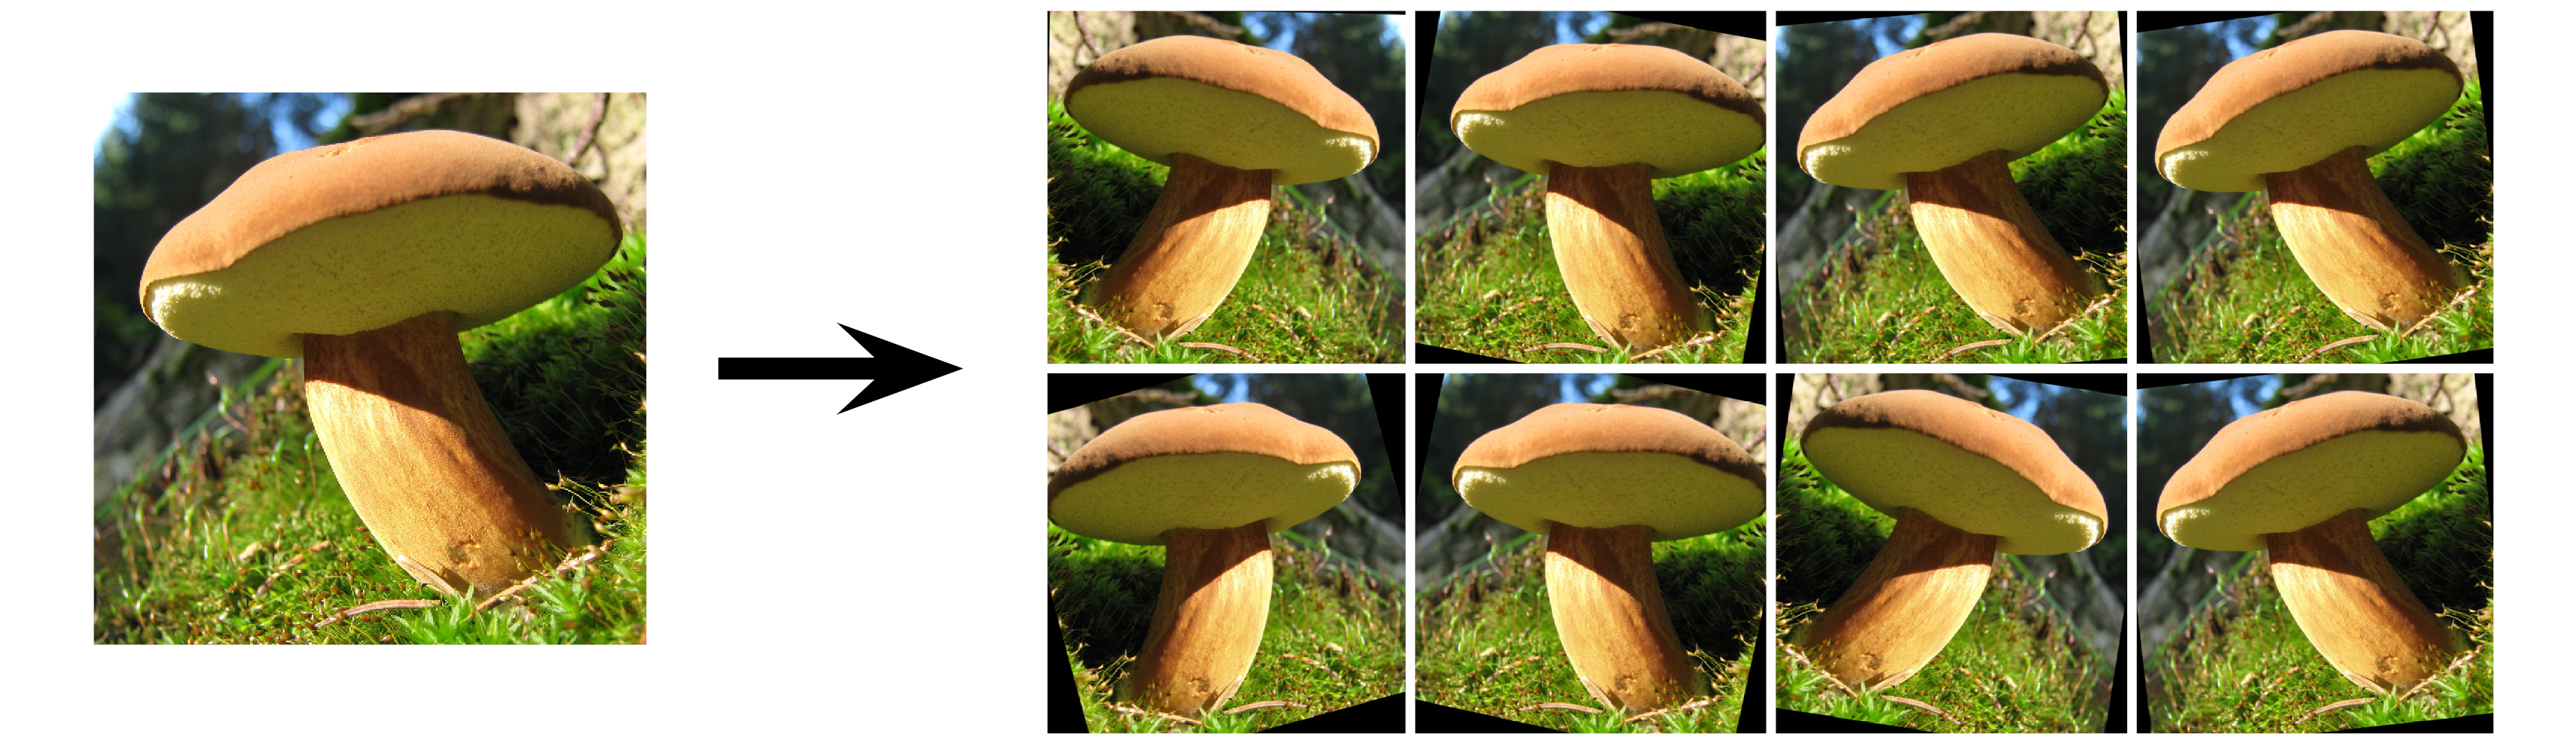
\includegraphics[width=0.8\textwidth]{augmented_data_1}
	\caption[Beispiel zu \textit{Data-Augmentation}]{\textit{Data-Augmentation} angewandt auf ein Bild}
	\label{img:da}
\end{figure}

\subsubsection{Zusatzinformationen sammeln \& aufbereiten} \label{cha:met:einf}
Da auch ein Experte für die akkurate Pilzartenbestimmung mehr als nur das Aussehen aus einer einzigen Perspektive benötigt, dürfte man dasselbe auch nicht von einem Bestimmungsalgorithmus erwarten. Deswegen sollen auch zusätzliche Informationen mit in die Bestimmung einfliessen können. Folgende Eingenschaften wurden aufgrund der einfachen Bestimmbarkeit und Implementierbarkeit in die Bestimmung aufgenommen:

\begin{table}[!htb]
	\def\arraystretch{1.2}
	\centering
	\begin{tabular}[t]{l | l }
		Eigenschaft & Optionen\\
		\hline
		Standort & Laubwald, Mischwald, Nadelwald, Wiese\\
		Durchmesser Hut/Fruchtkörper & klein ($<$3cm), mittel (3-10cm), gross ($>$10cm)\\
		Oberfläche Hut/Fruchtkörper & trocken, feucht\\
		Hutrand & glatt, wellig, gerieft, kein\\
		Sporenanlage & Lamellen, Röhren, Fruchtschicht, Fruchtmasse\\
		Lamellenhaltung & frei, herablaufend, angewachsen, kein\\
		Ring & hängend, aufsteigend, doppelt, gerieft, fleischig, kein\\
		Stiel & voll, wattig, hohl, kein\\
		Geruch & angenehm, geruchlos, stinkend
	\end{tabular}
	\caption{Zusatzinformationen für genauere Pilzartenbestimmung}
	\label{table:extra_inf}
\end{table}

Von den ausgewählten Pilzarten wurden diese Informationen mithilfe des Pilznachschlagewerks \textit{Welcher Pilz ist das?} von Markus Flück \cite{wpid} zusammengetragen. Eine Tabelle mit den Eigenschaften aller Pilzarten findet sich im Anhang (Tabelle \ref{table:shrooms_einf}).

Da die \textit{Deep Learning Toolbox} von Matlab nicht auf mehrere Eingangssignale ausgelegt ist, mussten diese Zusatzinformationen in den Bilddaten selber hinterlegt werden. Hierzu codiert jedes Pixel der ersten Bildzeile eine Option der Pilzeingenschaften. Wenn die Informationen einer Eigenschaft gegeben sind, nehmen die zu den Optionen entsprechenden Pixel Werte von 1 resp. -1 an; ist eine Information nicht gegeben, so werden diese Pixel auf den neutralen Wert 0 gesetzt. Mittels des benutzerdefinierten \textit{Extraction-Layers} können diese Informationen abgegriffen werden, um tiefer im Netz direkt verarbeitet werden zu können. Ein vor das \textit{KNN} geschaltete \textit{Cover-Layer} überschriebt diese Pixel der ersten Zeile, damit diese keinen Einfluss auf den Bilderkennungsteil haben.

\begin{figure}[h]
	\centering
	\includegraphics[width=0.8\textwidth]{einf_extraction}
	\caption[Extraktion und Einspeisung von Zusatzinformationen]{Extraktion und Einspeisung von Zusatzinformationen}
	\label{img:extr_layer}
\end{figure}
 
 
%Zusammengefasst ergeben sich aus der Datenbeschaffung und Datenaufbereitung folgende Zusammensetzung der Trainings- und Validierungsdaten:
%\begin{center}
%	\begin{tabular}{l | l | l | l | l}
%		Quelle & Training  & Training  & Validierung  & Validierung \\
%		  & bekannt & unbekannt & bekannt & unbekannt\\
%		\hline
%		SwissFungi & ca. 25 & 1840 & ca. 5 & 160\\
%		Webseite & ca. 15 & 0 & ca. 3 & 0\\
%		Crawler & ca. 130 & 0 & ca. 12 & 0\\
%		Video & ca. 75 & 0 & 0 & 0\\
%		\hline
%		\hline
%		& mind. 230
%	\end{tabular}
%\end{center}

\subsection{Entwicklungsprozess}\label{cha:met:dev}
Mit den aufbereiteten Trainingsdaten gilt es im nächsten Schritt den Algorithmus für die Pilzartenerkennung zu erarbeiten. In den folgenden Abschnitten wird beschrieben, welche Modifikationen zu einer signifikanten Verbesserung der Bestimmungsleistung beigetragen haben. Dabei wird in diesem Kapitel der Prozentsatz der richtig erkannten Validierungsdaten als Metrik für den Vergleich der Algorithmen verwendet. Durch \textit{Data-Augmentation} können z.T. auch unterschiedliche Resultate erhalten werden. Um trotzdem einen zuverlässigen Mittelwert für die Diskussion zu erhalten, werden die Validierungsdaten je zehn mal eingespeist und kategorisiert.

\subsubsection{Bezugswert}
Um bestimmen zu können, ob ein Algorithmus tatsächlich ''intelligentes'' Verhalten aufweist und nicht durch Zufall die korrekte Lösung errät, gilt es im ersten Schritt einen Richtwert für die Leistung zu finden. Diesen Wert gilt es von den Algorithmen zu übertreffen.
%Bei 21 Klassen kann durch zufälliges Zuteilen von Antworten eine Genauigkeit von $\frac{1}{21} \approx 4.76\%$ erreicht werden.
Mit den in Kapitel \ref{cha:met:preprocessing} gegebenen Klassenverhältnissen ist es naheliegend, jedes Bild der unbekannten Kategorie zuzuteilen. Mit dieser Strategie erhält man eine Genauigkeit von $\frac{8}{20+8} \approx$\textbf{28.6\%}, welcher als Bezugswert für den zu entwickelnden Algorithmus verwendet werden soll.

\subsubsection{Basis-SNN}
Der erste Algorithmus besteht aus einem einfachen \textit{SNN} mit einem \textit{Fully-Connected-Layer} als \textit{Hidden-Layer} und einem weiteren \textit{Fully-Connected-Layer} als \textit{Output-Layer}. Für das Training werden die zugeschnittenen Bilddaten nur mittels Bildnormalisierung vorverarbeitet; \textit{Data-Augmentation}, der Grünfilter sowie die Zusatzinformationen werden erst in den folgenden Abschnitten implementiert.

%Wie bereits im Kapitel \ref{cha:theo:dl} erwähnt worden ist, sollte theoretisch ein entsprechend grosser \textit{Hidden-Layer} für die korrekte Bestimmung aller Pilzbilder genügen.
Um ein grobes Bild der Leistung zu erhalten, werden folgende \textit{Meta-Parameter} des \textit{SNN}s variiert: Die Eingangsdatengrössen (200$\times$200px, 50$\times$50px oder 10$\times$10px\footnote{Skalierung der Bilder wird mittels \textit{bikubischer Interpolation} durchgeführt.}) sowie die \textit{Hidden-Layer}-Grösse ($20$, $60$ oder $100$ Neuronen). Für die restlichen \textit{Meta-Parameter} dienen vorerst Werte, welche sich erfahrungsgemäss für ähnliche Bilderkennungsprobleme bewährt haben. Alle \textit{Meta-Parameter} sind in der Tabelle \ref{table:basic_snn_training} im Anhang zu finden. Folgend die Ergebnisse:

\begin{table}[h]
	\begin{center}
		\def\arraystretch{1.4}
		\begin{tabular}{c | c | c | c }
			& \multicolumn{3}{l}{Anzahl \textit{Hidden-Neuronen}} \\
			Bildauflösung & 20 & 60 & 100\\
			\hline
			$200\times200$px& 3.6\%& 3.6\% & 3.6\%\\
			$50\times50$px& 12.5\% & 13.6\% & 20.4\%\\
			$10\times10$px& 41.3\% & \textbf{43.6\%} & 40.2\%\\
		\end{tabular}
	\end{center}
\caption[Bestimmungsleistung von \textit{SNN}s]{Bestimmungsleistung von \textit{SNN}s im einem \textit{Hidden-Layer}}
\label{table:snn}
\end{table}

Bemerkenswert ist das Ergebnis für das \textit{SNN} mit 60 \textit{Hidden-Neuronen}, welches die kleinsten Eingangsdaten erhalten hat: Mit nur 0.25\% der vorhandenen Daten leistet es mehr als das Zehnfache wie die Netze, welche alle 200$\times$200$\times$3 (Auflösung $\times$ Farbkanäle) Datenpunkte erhalten haben, und fast das Doppelte des Bezugswertes. Der nächste Schritt ist es nun, die Komprimierung der Informationen nicht durch verlustbehaftetes Skalieren\footnotemark[\value{footnote}] zu Erreichen, sondern durch Hinzufügen von zusätzlichen \textit{Convolution-Layers}.

\subsubsection{Basis-CNN}
Als Grundlage für das \textit{CNN}s dient ein nur aus \textit{Convolution-Layers}, \textit{Pooling-Layers} und einem \textit{Fully-Connected-Layer} (entspricht dem \textit{Output-Layer}) zusammengesetztes Netz (komplette Liste der \textit{Meta-Parameter} siehe Tabelle \ref{table:basic_cnn_training}). Als grobe Vorlage für Einstellungen der drei \textit{Convolution-Pooling-Einheiten} diente \textit{AlexNet}\cite{alexnet}. Die Auflösung der Eingangsdaten wird für das Training des \textit{CNN}s bei 200$\times$200px belassen, da die Filterung von den relevanten Informationen den \textit{Convolution-Layers} überlassen werden dann.

\begin{figure}[h]
	\centering
	\includegraphics[width=\textwidth]{baseline_cnn}
	\caption[Trainingsverlauf Basis-\textit{CNN}]{Trainingsverlauf vom Basis-{CNN}: Leistung mit Trainingsdaten in blau, Leistung mit Validierungsdaten in grau}
	\label{img:baseline_cnn}
\end{figure}

Nach dem Training erreichte das \textit{Basis-CNN} mit den Trainingsdaten eine Genauigkeit von 88.3\%. Mit den Testdaten etwa ein Drittel weniger: \textbf{56.1\%}. Wie in der Abbildung \ref{img:baseline_cnn} zu erkennen ist, verbessert sich die Leistung der Trainingsdaten (blau) kontinuierlich, die der Validierungsdaten (grau) jedoch stagniert ab Epoche 8 (Iteration 600). Dies ist ein typisches Verhalten eines überangepassten Algorithmus(siehe \textit{Überanpassung} in Kapitel \ref{cha:theo:ml:b-v}).


\subsubsection{Data-Augmentation} \label{cha:met:da}

\begin{figure}[]
	\centering
	\includegraphics[width=\textwidth]{dataaug}
	\caption[Trainingsverlauf Basis-\textit{CNN} mit \textit{Data-Augmentation}]{Trainingsverlauf vom Basis-{CNN} mit \textit{Data-Augmentation}: Leistung mit Trainingsdaten in blau, Leistung mit Validierungsdaten in grau}
	\label{img:dataaug_cnn}
\end{figure}

Um der Überanpassung von Basis-\textit{SNN} aus dem letzten Abschnitt entgegenzuwirken, sollen die durch \textit{Data-Augmentation} künstlich erweiterten Trainingsdaten verwendet werden. Alle Einstellungen zur \textit{Data-Augmentation} sowie \textit{Meta-Parameter} sind in der Tabelle \ref{table:dataaug_training} im Anhang zu finden.

Nur mit künstlich erweiterten Trainingsdaten erreichte das ansonsten gleiche \textit{CNN} eine Leistung von \textbf{63.4\%}. Zudem ist in Abbildung \ref{img:dataaug_cnn} auch deutlich zu erkennen, dass die Differenz zwischen Validierungsdaten und Trainingsdaten (67.2\%) massiv kleiner ist.

\subsubsection{Farbfilter}
Der folgende Testlauf wird mit den selben \textit{Meta-Parameter} wie \textit{CNN} aus \ref{cha:met:da} ausgeführt, jedoch wurde auf alle Eingangsdaten der im Kapitel \ref{cha:met:gf} eingeführte Grünfilter angewandt.

Nach dem Training  erreichte man ein ähnliches Resultat wie ohne Filter (60.71\%), jedoch unterschieden sich die Methoden in der Laufzeit: Das Filtern der Grün-Töne für jedes Trainingsexemplar verdoppelte fast die Berechnungszeit (45 gegenüber 27 Minuten).

%\begin{figure}[h]
%	\centering
%	\includegraphics[width=\textwidth]{dataFilter}
%	\caption[Trainingsverlauf Basis-\textit{CNN} mit Grün-Filter]{Trainingsverlauf vom Basis-{CNN} mit Grün-Filter: Leistung mit Trainingsdaten in blau, Leistung mit Validierungsdaten in grau}
%	\label{img:gf_cnn}
%\end{figure}

Aus dem ähnlichen Ergebnis lässt sich schliessen, dass das \textit{CNN} die für die Bestimmung relevanten Farben ohne externer Unterstützung filtern kann, was wiederum auf eine robuste Netzarchitektur deutet. Aufgrund des grossen zusätzlichen Zeitaufwandes wird diese Massnahme nicht in den folgenden \textit{CNN}s implementiert.

\subsubsection{Justierung des CNNs}\label{cha:met:adjcnn}
Da die \textit{Meta-Parameter} des Basis-\textit{CNN}s nur durch eine erfahrungsgestützte Schätzung eingestellt worden sind, gilt es in diesem Abschnitt die \textit{Meta-Parameter} zu justieren. Dabei sollen weitere \textit{Layers} und \textit{Layer-}Typen verwendet werden, um das \textit{CNN} weiter auf die Pilzartenerkennung zu spezialisieren. Da es für die Zusammenstellung sowie Einstellung von \textit{Layern} unzählige Kombinationsmöglichkeiten gibt, soll nur ein kleiner Bereich möglichst systematisch untersucht werden.

Eine erste signifikante Verbesserung wurde durch die Erweiterung jeder \textit{Convolution-Pooling-Einheit} mit je einem \textit{ReLU-} sowie \textit{Batch-Normalization-Layer} erreicht (68.2\%). Durch weitere Exploration des Parameterraumes konnten durch Anpassung der \textit{Feature-Map}-Anzahl noch 6 weitere Prozentpunkte gewonnen werden, was sich zu einem finalen Ergebnis von \textbf{74.6\%} summiert. Zu beachten gilt es jedoch auch das Resultat der Trainingsdaten (90.6\%), welche auf eine ausgeprägte Überanpassung deutet. Folgende \textit{Meta-Parameter} wurden verwendet:


\begin{table}[!htb]
	\def\arraystretch{1.2}
	\centering
	\begin{subtable}[t]{.5\linewidth}
		\begin{tabular}[t]{l | l }
			\multicolumn{2}{c}{\textbf{Trainings-Einstellungen}}\\
			\hline
			\textit{Parameter} & Wert\\
			\hline
			\hline
			Lernrate $\eta$ & Epochen 1-10: 0.01\\
					        & Epochen 11-20: 0.001\\
			Mini-Batch-Grösse & 128\\
			Anz. Lernepochen & 20\\
			L2 Regularisierung & 0.002\\
			Trainingsdaten mischen& nach Epoche\\
			Bildnormalisierung & \checkmark\\
			\textit{Data-Augmentation}& Drehung: $\pm25^{\circ}$ \\
			& X-Versetzung: $\pm10px$ \\
			& Y-Versetzung: $\pm10px$ \\
			& X-Spiegelung: \checkmark \\
			& Y-Spiegelung: $\times$ \\
			Zusatzinformationen &  $\times$ \\
		\end{tabular}
	\end{subtable} 
	\caption{Trainings-Parameter des justierten \textit{CNN}s}
	\label{table:final_cnn_training}
\end{table}

\begin{table}[!htb]
	\def\arraystretch{1.4}
	\centering
	\begin{subtable}[t]{.55\linewidth}
		\begin{tabular}[t]{l | l }
			\multicolumn{2}{c}{\textbf{Netzaufbau}}\\
			\hline
			\textit{Layer}-Typ & Grösse\\
			\hline
			\hline
			Bildeingabe-\textit{Layer} & 200$\times$200$\times$3\\
			\hline
			\textit{Convolution-Layer}& Filter: 10 $\times$ 10\\
			& Schrittweite: 4\\
			& Anz. \textit{Feature Maps}: 40\\
			\hline
			\textit{ReLU-Layer} \& & \\
			\textit{Batch-Norm.-Layer} & \\
			\hline
			\textit{max-Pooling-Layer}& Filter: 3 $\times$ 3\\
			& Schrittweite: 2\\
			
			\hline
			\textit{Convolution-Layer}& Filter: 5 $\times$ 5\\
			& Schrittweite: 1\\
			& Anz. \textit{Feature Maps}: 80\\
			\hline
			\textit{ReLU-Layer} \& & \\
			\textit{Batch-Norm.-Layer} & \\
			\hline
			\textit{max-Pooling-Layer}& Filter: 3 $\times$ 3\\
			& Schrittweite: 2\\
			\hline
			\textit{Convolution-Layer}& Filter: 2 $\times$ 2\\
			& Schrittweite: 1\\
			& Anz. \textit{Feature Maps}: 100\\
			\hline
			\textit{ReLU-Layer} \& & \\
			\textit{Batch-Norm.-Layer} & \\
			\hline
			\textit{max-Pooling-Layer}& Filter: 2 $\times$ 2\\
			& Schrittweite: 2\\
			\hline
			\textit{Output-Layer}   & 21\\
		\end{tabular}
	\end{subtable}%
	\caption{Aufbau des justierten \textit{CNN}s}
	\label{table:final_cnn_structure}
\end{table}

\subsubsection{Transfer-Learning}\label{cha:met:tl}
In Kapitel \ref{cha:theo:mod:tl} wurde erwähnt, dass bereits vortrainierte \textit{CNN}s auch auf neue Datensätze umtrainiert werden können. Im Rahmen dieser Arbeit sollen daher zwei hochperformante \textit{CNN}s der Bilderkennung auf das Pilzartenerkennungsproblem für \textit{Transfer-Learning} verwendet werden: AlexNET\cite{alexnet} und GoogLeNet\cite{googlenet}. Beides sind Ergebnisse der \textit{ImageNet Large Scale Visual Recognicion Challenge}\cite{ilsvrc} und wurden mit etwa 1.2 Millionen verschiedenen Trainingsbildern auf 1000 verschiedene Kategorien trainiert.

Um AlexNET resp. GoogLeNet auf das Pilzerkennungsproblem anzupassen, musste nur der letzte \textit{Fully-Connected-Layer} (\textit{Output-Layer}) ersetzt werden durch einen \textit{Fully-Connected-Layer} mit 21 Neuronen. Für \textit{Transfer-Learning} empfiehlt es sich zudem, etwas modifizierte Trainingseinstellungen zu verwenden: Der neue \textit{Output-Layer} soll einiges stärker trainiert werden als die transferierten \textit{Layer} aus dem trainierten Netz, weswegen die Lernraten $\eta$ individuell auf 20 (\textit{Output-Layer}) resp. 0.0001 (transferierte \textit{Layer}) gesetzt werden. In Tabelle \ref{table:transfer_training} sind nochmals alle \textit{Meta-Parameter} aufgelistet.

\begin{table}[!htb]
	\def\arraystretch{1.4}
	\centering
	\begin{subtable}[t]{.5\linewidth}
		\begin{tabular}[t]{l | l }
			\multicolumn{2}{c}{\textbf{Netzaufbau}}\\
			\hline
			\textit{Layer}-Typ & Grösse\\
			\hline
			\hline
			Bildeingabe-\textit{Layer} & AlexNET:\\
									   & 227$\times$227$\times$3\\
									   & GoogLeNet:\\
									   & 224$\times$224$\times$3\\
			\hline
			transferierte \textit{Layers}& AlexNET: 21 \textit{Layers}\\
										& GoogLeNet: 25 \textit{Layers}\\
			\hline
			\textit{Output-Layer}   & 21\\
		\end{tabular}
	\end{subtable}%
	\begin{subtable}[t]{.5\linewidth}
		\begin{tabular}[t]{l | l }
			\multicolumn{2}{c}{\textbf{Trainings-Einstellungen}}\\
			\hline
			\textit{Parameter} & Wert\\
			\hline
			\hline
			Lernrate $\eta$ & \textit{Output-Layer}: 20 \\
			& transferiert: 0.0001\\
			Mini-Batch-Grösse & 64\\
			Anz. Lernepochen & 6\\
			L2 Regularisierung & 0.0001\\
			Trainingsdaten mischen& nach Epoche\\
			Bildnormalisierung & \checkmark\\
			\textit{Data-Augmentation}& Drehung: $\pm25^{\circ}$ \\
									& X-Versetzung: $\pm10px$ \\
									& Y-Versetzung: $\pm10px$ \\
									& X-Spiegelung: \checkmark \\
									& Y-Spiegelung: $\times$ \\
									Zusatzinformationen &  $\times$ \\
		\end{tabular}
	\end{subtable} 
	\caption[\textit{Meta-Parameter} \textit{Transfer-Learning}]{\textit{Meta-Parameter} für \textit{Transfer-Learning}}
	\label{table:transfer_training}
\end{table}

Durch die vortrainierten \textit{CNN}s konnten wieder signifikant bessere Ergebnisse erzielt werden: Das mit AlexNET modifizierte \textit{CNN} erreichte eine Genauigkeit von 83.8\%, das mit GoogLeNet modifizierte sogar \textbf{84.3\%}.

Wie im Trainingsverlauf des \textit{GoogLeNet-Transfer-CNN}s (Abbildung \ref{img:transfer_cnn}) zu erkennen ist, leidet dieses \textit{CNN} im Gegensatz zum dem aus vorherigem Abschnitt in keiner Weise an Überanpassung.

\begin{figure}[h]
	\centering
	\includegraphics[width=\textwidth]{transfer_google_2}
	\caption[Trainingsverlauf \textit{Transfer-Learning}]{Trainingsverlauf von \textit{Transfer-Learning} mit GoogLeNet: Leistung mit Trainingsdaten in blau, Leistung mit Validierungsdaten in grau}
	\label{img:transfer_cnn}
\end{figure}

\subsubsection{Einspeisung von Zusatzinformationen} \label{cha:met:einfimpl}
Bis jetzt konnten schon eindrückliche Ergebnisse erzielt werden, wenn man betrachtet, dass für die Bestimmung nur mit den Informationen eines Bildes gearbeitet wurde. Um die Fehlerquote weiter einzugrenzen, sollen die in Kapitel \ref{cha:met:einf} eingeführten Zusatzinformationen mit in die Pilzartenbestimmung mit einfliessen. Hierfür wird das im vorherigen Abschnitt erarbeitete \textit{GoogLeNet-Transfer-CNN} mit dem \textit{Information-Extraction-} und \textit{Information-Cover-Layer} so modifiziert, damit die in den Eingangsbildern enthaltenen Zusatzinformationen direkt im \textit{fully-connected} \textit{Output-Layer} verarbeitet werden können (vgl. Abbildung \ref{img:extr_layer}). Da der \textit{Output-Layer} standardmässig Bildinformationen von über Eintausend Neuronen des letzten transferierten \textit{Layers} erhält, wurden die vergleichsweise wenigen Neuronen der Zusatzinformationen (34) in ihrer Anzahl verzehnfacht, um in der Unmenge an Bildinformationsneuronen schneller als wichtige Informationsträger detektiert zu werden.

Um das \textit{CNN} nicht primär von den Zusatzinformationen abhängig zu machen, werden diese nicht immer zu Verfügung gestellt. Um dies zu bewerkstelligen, werden 50\% der Trainingsexemplare ganz ohne Zusatzinformationen eingespeist, 10\% erhalten die Informationen aller Eigenschaften und für die restlichen 40\% der Bilder werden zwischen 1 und 10 der 11 Eigenschaften angegeben.

Alle \textit{Meta-Parameter} finden sich in folgender Tabelle:

\begin{table}[!htb]
	\def\arraystretch{1.4}
	\centering
	\begin{subtable}[t]{.5\linewidth}
		\begin{tabular}[t]{l | l }
			\multicolumn{2}{c}{\textbf{Netzaufbau}}\\
			\hline
			\textit{Layer}-Typ & Grösse\\
			\hline
			\hline
			Bildeingabe-\textit{Layer} & 224$\times$224$\times$3\\
			\hline
			\textit{Extraction-Layer} & Abgreifen von 34 \\
			  & Zusatzinformationen\\
			\hline
			transferierte \textit{Layers}& GoogLeNet: 25 \textit{Layers}\\\hline
			\textit{Extraction-Layer} & Einspeisung und\\
			& Verzehnfachung der\\
			& Zusatzinformationen\\
			\hline
			\textit{Output-Layer}   & 21\\
		\end{tabular}
	\end{subtable}%
	\begin{subtable}[t]{.5\linewidth}
		\begin{tabular}[t]{l | l }
		\multicolumn{2}{c}{\textbf{Trainings-Einstellungen}}\\
		\hline
		\textit{Parameter} & Wert\\
		\hline
		\hline
		Lernrate $\eta$ & \textit{Output-Layer}: 20 \\
		& transferiert: 0.0001\\
		Mini-Batch-Grösse & 48 (GPU-Limitation)\\
		Anz. Lernepochen & 11\\
		L2 Regularisierung & 0.0001\\
		Trainingsdaten mischen& nach Epoche\\
		Bildnormalisierung & \checkmark\\
		\textit{Data-Augmentation}& Drehung: $\pm25^{\circ}$ \\
		& X-Versetzung: $\pm10px$ \\
		& Y-Versetzung: $\pm10px$ \\
		& X-Spiegelung: \checkmark \\
		& Y-Spiegelung: $\times$ \\
		Zusatzinformationen & keine: 50\%\\
							 &teilweise: 40\%\\
							 &alle: 10\%
		\end{tabular}
	\end{subtable} 
	\caption[]{\textit{Meta-Parameter} für \textit{Transfer-Learning} mit GoogLeNet und Zusatzinformationen}
	\label{table:extra_transfer}
\end{table}

Durch die unzuverlässige Einspeisung der Zusatzinformationen konnte die Lücke zur 100\%-Marke doch noch halbiert werden: Das finale Trainingsresultat für dieses \textit{CNN} beläuft sich auf \textbf{92.3\%} Genauigkeit. Da das \textit{CNN} auch die Trainingsdaten mit 93.8\% Genauigkeit erkennt, kann auf eine sehr geringen Überanpassung gedeutet werden. Diese finale Version wie auch die zwei Vorgänger werden als Ergebnis dieser Arbeit genauer analysiert.





%\subsubsection{CNN-Ensemble}